\documentclass{SMR}
%graphics
\graphicspath{ {/Where/you/keep/your/graphics} }  % <- UPDATE THE PATH

%who and where
\smrtitle{SMR.cls}
\smrauthor{Marcin and Nick}
\smraffiliation{Edinburgh and Glasgow Universities}

\title{Scottish Music Review class file for PDFLaTeX}
\author{Pietryszwski, Marcin \and Bailey, Nick}

\begin{document}

\maketitle

\begin{abstract}
A class for the Scottish Music Review
\end{abstract}

\section{Section One - comment out if not needed} %section title comes here,
                                                  %comment out if there are
                                                  %no sections in the article 
The usual title, author and date commands given in the preamble
are used to head up the paper, but there's also the smr- varients
which get used in the headers.

If you don't supply them it'll still work, but you'll be warned.

If you supply an smrauthor, you \emph{must} supply an affiliation.

The title is set at the top left of left-hand pages, and the
author above the affiliation at the top right of right-hand pages.

\vspace*{1.0cm}

Here is some text to be formatted followed by a figure of
a Klein Bottle as an example of how graphics are formatted
in this template.

\begin{figure}[h]
\caption{Klein Bottle} %EDIT CAPTION
\centering
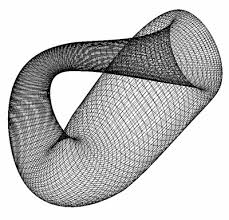
\includegraphics[width=0.5\textwidth]{klein.jpg}
\end{figure}

Here is some text following a figure with a footnote added
to it \footnote{I am a footnote}. Here is an \emph{emphasized text}
followed by \textbf{bold text} which can be used for
\textbf{[Referencing]}

\pagebreak

\subsection{A Subsection} %subsections

Subsections are numbered per section.

\section{A New Section}

This section has its own subsection.

\subsection{Another subsection}

Like this one.

You will find the bibliography on the next page.
\vfill\pagebreak

%a separate section for bibliography

\section*{Bibliography}

\end{document}
